\chapter{Атом гелия}

\section{Атом гелия. Спиновые функции двух электронов. Пара- и ортосостояния}

\begin{figure}[h!]
\centering
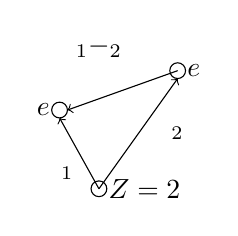
\begin{tikzpicture}[domain=-3:3]
  \draw (0, 0) circle (1mm) node [right] {$Z=2$};  
  \draw (-0.5, 1) circle (1mm) node [left] {$e$};  
  \draw (1, 1.5) circle (1mm) node [right] {$e$};  
  \draw[<-] (-0.5, 0.9) -- (0, 0);
  \node at (-0.4, 0.2) {$\vr_1$};
  \draw[<-] (1, 1.4) -- (0, 0) ;
  \node at (1, 0.7) {$\vr_2$};
  \draw[<-] (-0.4, 1) -- (1, 1.5);
   \node at (0, 1.8) {$\abs{\vr_1 - \vr_2}$};
\end{tikzpicture}
\caption{Атом гелия.} \label{fig:17_1}
\end{figure}


Запишем гамильтониан для атома гелия:
\begin{equation}
\label{eq:17_1_1}
\op{H} = \frac{\op{\vp}_1^2}{2m} - \frac{Ze^2}{r_1} + \frac{\op{\vp}_2^2}{2m} - \frac{Ze^2}{r_2} + \frac{e^2}{\abs{\vr_1 - \vr_2}}
\end{equation}

\begin{equation}
\label{eq:17_1_2}
\op{H} \Psis(\xi_1, \xi_2) =E\Psis(\xi_1, \xi_2)
\end{equation}

Мы находимся в рамках релятивистского приближения $\brc{\frac{v}{c}}^2 \ll 1$.

$$
\Psis(\xi_1, \xi_2) = \Phi(\vr_1, \vr_2) \chi(\sigma_1, \sigma_2)
$$

Из главы XVI, \S1:
$$
\Psis_1 = \Phi^S(\vr_1, \vr_2) \chi^A(\sigma_1, \sigma_2)
$$
$$
\Psis_2 = \Phi^A(\vr_1, \vr_2) \chi^S(\sigma_1, \sigma_2)
$$

Из упр. 2 II задания мы знаем собственные функции системы из двух частиц со спинами $\frac{1}{2}$.
$$
s_1=\frac{1}{2}, ~ s_2=\frac{1}{2}~~~~~\op{\vec{s}} = \op{\vec{s}} _1 + \op{\vec{s}}_2
$$

Из правила \eqref{eq:15_2_4}:
$$
s = \abs{s_1 - s_2}, \abs{s_1 - s_2} + 1, ..., s_1+s_2 
$$

В нашем случае $s = 0, 1$.

Найдем собственные векторы $\ket{s s_z}$ операторов $\op{\vec{s}}^2$, $\op{s}_z$, $\op{\vec{s}}_1^2$, $\op{\vec{s}}_2^2$.

$$
s = 0, s_z = 0 \text{    или    } s = 1, s_z=-1, 0, 1
$$

Выпишем собственные функции:
$$
\chi(0, 0) = \frac{1}{\sqrt{2}}\brc{\alpha(1)\beta(2) - \beta(1)\alpha(2)}
$$

- синглетная спиновая волновая функция <<S>>.

\begin{gather*}
\chi(1, 1) = \alpha(1)\alpha(2) \\
\chi(1, 0) = \frac{1}{\sqrt{2}}\brc{\alpha(1)\beta(2) + \beta(1)\alpha(2)} \\
\chi(1, -1) = \beta(1)\beta(2)
\end{gather*}

- триплетная спиновая волновая функция <<T>>.

$\chi^S(\sigma_1, \sigma_2)$ - симметричная волновая функция, $s = 1$.

$\chi^A(\sigma_1, \sigma_2)$ - антисимметричная волновая функция, $s = 0$.

Состояние с $s = 0$ - парагелий - синглетные уровни.

Состояние с $s = 1$ - ортогелий - триплетные уровни.

Переход между парагелием и ортогелием запрещен правилами отбора т.к. $\Delta S \not = 0$.

В макроскопическом масштабе гелий -- <<два индивидуальных вещества>>.

\section{Обменное взаимодействие}

В \eqref{eq:17_1_2}
\begin{gather*}
\op{H} = \op{H}^\zr + \op{V} \\
\op{H}^\zr = \op{H}_1 + \op{H}_2 \\
\op{H}_i = \frac{\op{\vp_i}^2}{2m} - \frac{Ze^2}{r_i} \\
\op{V} = \frac{e^2}{\abs{\vr_1 - \vr_2}}
\end{gather*}

$\nu_1 = (n_1, l_1, m_1)$, $\nu_2 = (n_2, l_2, m_2)$ - мультииндексы.

Если $\nu_1 \not = \nu_2$, то такие электроны называются неэквивалентными.

Если $\nu_1 = \nu_2$, то такие электроны называются эквивалентными.

Запишем пространственную часть волновой функции.

\begin{gather}
\label{eq:17_2_1}
\Phi^{A, S}(\vr_1, \vr_2) = \frac{1}{\sqrt{2}}\brcr{\phi_{\nu_1}(\vr_1) \phi_{\nu_2}(\vr_2) \mp \phi_{\nu_2}(\vr_1) \phi_{\nu_1}(\vr_2)}, ~~~\nu_1 \not = \nu_2 \nonumber \\
\Phi^S(\vr_1, \vr_2) = \phi_{\nu}(\vr_1) \phi_{\nu}(\vr_2), ~~~\nu_1 = \nu_2= \nu
\end{gather}

Воспользуемся выводами \S 1 главы XVI. Возможные волновые функции:

\begin{equation}
\label{eq:17_2_2}
\underbrace{\Phi^S \chi(0, 0)}_{s = 0}~~~\underbrace{\Phi^A \chi(1,1)~~~\Phi^A \chi(1,0)~~~\Phi^A \chi(1,-1)}_{s = 1}
\end{equation}

Запишем энергию в нулевом порядке ТВ:
$$
E_{\nu_1, \nu_2}^\zr = E_{\nu_1} + E_{\nu_2} = E_{n_1} + E_{n_2}
$$

Если  $\nu_1 = \nu_2= \nu$, то $\Phi^A \equiv 0$ и возмущение дает сдвиг для $E_{\nu \nu}^\one$.

Если  $\nu_1 \not = \nu_2$, то
\begin{equation}
\label{eq:17_2_3}
\boxed{E_{\nu_1 \nu_2}^\one = \bfk{\Phi^{A, S}}{\op{V}}{\Phi^{A, S}} = J_{\nu_1 \nu_2} \pm K_{\nu_1 \nu_2}} 
\end{equation}

Знак + соответствует $s = 0$, - -- $s = 1$.

\begin{gather}
\label{eq:17_2_4}
J_{\nu_1 \nu_2} = \int \int d\vr_1 d\vr_2 \abs{\phi_{\nu_1}(\vr_1)}^2 \abs{\frac{e^2}{\vr_1 - \vr_2}} \abs{\phi_{\nu_2}(\vr_2)}^2 = \int \int d\vr_1 d\vr_2 \abs{\phi_{\nu_1}(\vr_1)}^2 \frac{e^2}{\abs{\vr_1 - \vr_2}} \cdot \nonumber \\ \cdot \abs{\phi_{\nu_2}(\vr_2)}^2
\end{gather}

- кулоновский интеграл. $e\rho_{\nu_1}(\vr_1) \times e\rho_{\nu_2}(\vr_2)~(e < 0)$.
$$
J_{\nu_1 \nu_2} > 0
$$

\begin{gather}
\label{eq:17_2_5}
K_{\nu_1 \nu_2} = \int \int d\vr_1 d\vr_2 \phi^*_{\nu_1}(\vr_1) \phi_{\nu_2}(\vr_1)\frac{e^2}{\abs{\vr_1 - \vr_2}}  \phi^*_{\nu_2}(\vr_2) \phi_{\nu_1}(\vr_2) = \nonumber \\
= \int \int d\vr_1 d\vr_2 \phi^*_{\nu_2}(\vr_1) \phi_{\nu_1}(\vr_1)\frac{e^2}{\abs{\vr_1 - \vr_2}}  \phi^*_{\nu_1}(\vr_2) \phi_{\nu_2}(\vr_2)
\end{gather}

- обменный интеграл.

$$
K_{\nu_1 \nu_2} > 0
$$

(доказательство в п. 15.43 [4]).

Из \eqref{eq:17_2_3}:

\begin{gather*}
E_{\nu\nu}^\one = J_{\nu\nu} \\
E_{\nu_1 \nu_2}^{(1), s=0} = J_{\nu_1\nu_2} + K_{\nu_1\nu_2} \\
E_{\nu_1 \nu_2}^{(1), s=1} = J_{\nu_1\nu_2} - K_{\nu_1\nu_2} 
\end{gather*}